%% ================================================================================
\chapter{Theory}
\label{ch:theory}
%% ================================================================================
The theory chapter. These are references \cite{aPaper}, \cite{aThesis}, \cite{aWiki}. Figure \ref{fig:dummy} shows a placeholder. 

\begin{figure}
  \centering
  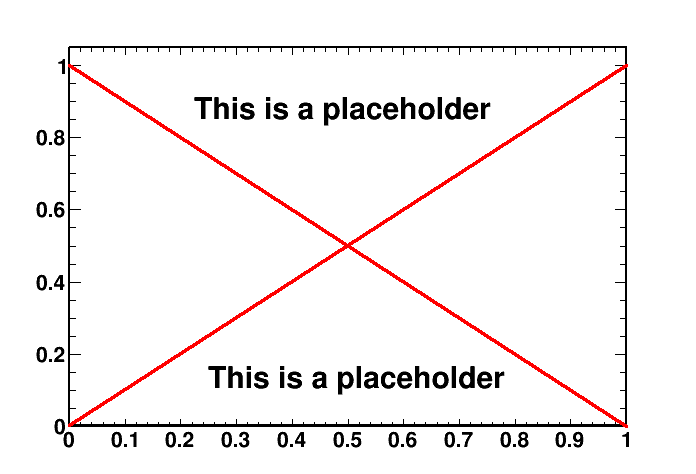
\includegraphics[width=.9\linewidth]{pic/dummy.png}
  \caption{This is a dummy plot.}
  \label{fig:dummy}
\end{figure}

\section{A section}
\label{sec:section}
Here we have Section \ref{sec:section}. \todo{This is a TODO marker} You might need this.


\section{Physic of cosmic rays}


\subsection{Creation of CR}
%		-supernovae (SNR)
%		-extra-galactic
%		-pulsars


\subsection{Propagation of CR}
%Propagation through the galaxy
%	-random B field -> no way to backtrace a CR
%	-interaction, shocks in MC
%	-Diffusion coefficient
%		-Can be different in disk, bubbles, or outside
%	-different diffuse coef mean different densities
%		-in MC, bubbles, outside
%		-can observe this inhomogeiniies via gamma rays

Once they are emitted, the cosmic rays propagate through the galaxy under the influence of different interactions.
The first one to notice is the complex manetic field created by all sorts of objects, from the stars to molecular clouds or any distribution of charged particles. It is not particularly strong \todo{put values} compared to the heliosphere or what we can create on Earth, but its very large scale suffice to bend the CR's path in all direction until the point where it is impossible to backtrace its origin.
An other possible interaction is the collisions with other particules. It will obviously depends on the density distribution of those colliders in the galaxy. We can expect a higher number of those in the disk, where the density of molecular clouds the highest.

All these influences can be modeled by a diffusion model, mainly defined by its diffusion coefficient, which discribes the average distance traveled in a certain time. The higher the coefficient, the faster a particule will diffuse in the galaxy. Each phenomenon can be attributed one of those coefficient to describe its effect on the cosmic rays. \todo{give values for Dmag, Dcoll...}
While the diffusion coefficient for the galactic magnetic field can be taken as constant throughout the milky way, the diffusion coefficient due to collision is proportional to the particles density. We can then expect a smaller coefficient in molecular clouds, where the density can reach \todo{value!}.

This coefficient ill also define the cosmic ray densities in various locations of the galaxy.

\subsection{Gamma-ray creation}
%		-pion decay
%		-bremmstrahlung
%		-inverse compton



\section{What are the unresolved problems of the precedent chapter}
%What are the unresolved problems of the precedent chapter:
%	-Spherical gamma-ray excess in GC when fitting spatial templates
%		-DM studies
%			-Hooper
%			-others...
%		-MSP studies
%			-Fermi
%			-Hooper
%			-Weniger
%
%	-High energy tail flux too hard
%	-Bad fits in bubbles and disk










